\documentclass[12pt,a4paper,oneside]{book} 
\usepackage{geometry}\geometry{left=2.5cm,right=2.5cm,top=2.5cm,bottom=2.5cm}

\usepackage{amssymb,amsmath}
\usepackage{fontspec}
\usepackage{zhspacing}
\usepackage[]{titlesec}
\titleformat{\chapter}{\centering\Huge\bfseries}{\thechapter}{1em}{}
\titleformat{\section}{\large\bfseries}{\thesection}{1em}{}
%\usepackage{graphicx}
\usepackage[subfigure]{graphfig}
\usepackage{fontspec,xunicode,xltxtra,verbatim}
\setromanfont[BoldFont={"[simhei.ttf]"}]{"[simsun.ttc]"}

\usepackage[pagewise]{lineno}


\usepackage{setspace}
\onehalfspacing
\usepackage[unicode=true,
 bookmarks=true,bookmarksnumbered=true,bookmarksopen=true,bookmarksopenlevel=1, 
 breaklinks=false,pdfborder={0 0 1},backref=section,colorlinks=true]
 {hyperref}


 
\makeatletter
\let\@afterindentfalse\@afterindenttrue
\@afterindenttrue
\makeatother
\setlength{\parindent} {2em}%中文缩进两个汉字位
 
 
 
\usepackage{listings}
\lstloadlanguages{C,C++,matlab} %程序清单关键字宏包
\lstset{xleftmargin=2em,xrightmargin=2em,breaklines=true,showstringspaces=false,keepspaces=true,aboveskip=1em}

\renewcommand\figurename{图}

\setmainfont{Adobe Song Std}
\begin{document}
\thispagestyle{empty}%本页无页码
\setcounter{chapter}{4} 
\chapter{基于相关的图像匹配算法}
\section{实验目的}
使用VS2008开发工具,c\#编程语言条件下,实现基于相关的图像匹配算法的图像操作。
\section{算法原理}

本实验提供三张图片,patterns.bmp包含12种不同的图案模式对应图(a),pat1.bmp对应图(b),pat2.bmp对应图(c),要在(a)中找到(b)和(c)中的子图像的最佳匹配。(b)中的图像对应(a)中第2行的第2个小图案,但整体亮度较其在(a)中更暗,(c)中图像则与(a)中第3行第2个小图案相似,略有细节不同。
\begin{Figure}[h]{基于相关的图像匹配}[label]
\begin{minipage}[t]{0.5\linewidth}
\centering
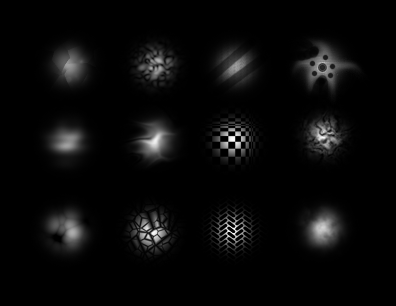
\includegraphics[width=2.2in]{patterns.png} 
\label*{\\a}
\end{minipage}%
\begin{minipage}[t]{0.3\linewidth}
\centering

\includegraphics[width=0.5in]{pat1.png} 
\label*{\\b}
\end{minipage}
\begin{minipage}[t]{0.15\linewidth}
\centering

\includegraphics[width=0.5in]{pat2.png} 
\label*{\\c}
\end{minipage}
%\graphfile[30]{patterns.png}  
\end{Figure}

在一个原始图片中查找最相似的模板图片,通过遍历原始图像素,与模板相素进行相关运算,相关值最大的位置即为匹配的坐标。
相关运算与卷积运算类似,需要对应分量相乘求和,但卷积是对模板进行了180的翻转;在计算过程中对模值进行了归一化,其实际是计算了向量的夹角。

使用的相关计算公式如下:
\begin{displaymath}
r(x,y)=\frac{
\sum_{s=0}^{K}\sum_{t=0}^{J}w(s,t)f(x+s,y+t))
}{
\left[
\sum_{s=0}^{K}\sum_{t=0}^{J}w^{2}(s,t)\cdot\sum_{s=0}^{K}\sum_{t=0}^{J}f^{2}(x+s,y+t))
\right]^{1/2}
}
\end{displaymath}

程序是窗体应用程序,使用线程进行运算,线程在运算完毕后,将结果通知给主窗体。

\section{实验过程}

\begin{enumerate}
\item 新建窗体应用程序。
\item 在项目中添加一个新类DataClass
\hspace*{0em}public static class DataClass\\
\hspace*{2em}\{\\
\hspace*{4em}public static MemoryStream ms\_bmp\_src, ms\_bmp\_result, ms\_bmp\_temp;\\
\hspace*{4em}public static Bitmap bp\_1;//原始大图\\
\hspace*{4em}public static Bitmap bp\_2;//模板\\
\hspace*{4em}public static bool bm\_ready; \\
\hspace*{4em}public static IntPtr frm1\_wnd\_handle;\\
\hspace*{4em}public const int GRAY\_FINISHED = 0x501;\\
\hspace*{2em}\}\\
\item 在Program.cs文件修改系统启动代码如下\\
\hspace*{4em}		static void Main()\\
\hspace*{4em}\{\\
\hspace*{6em}Application.EnableVisualStyles();\\
\hspace*{6em}Application.SetCompatibleTextRenderingDefault(false);\\
\hspace*{6em}Form1 frm1 = new Form1();\\
\hspace*{6em}DataClass.frm1\_wnd\_handle = frm1.Handle;\\
\hspace*{6em}DataClass.ms\_bmp\_src = new MemoryStream(5000000);\\
\hspace*{6em}DataClass.ms\_bmp\_result = new MemoryStream(5000000);\\
\hspace*{6em}DataClass.ms\_bmp\_temp = new MemoryStream(1000000); \\
\hspace*{6em}Application.Run(frm1);\\
\hspace*{4em}\}\\
\item 设计窗体界面,在界面上添加三个图片框,图片框为并排排列,三个按扭竖向排列,可参考最后的运行结果图。
\item 加入全局变量声明\\
\hspace*{4em}[DllImport("User32.dll", EntryPoint = "SendMessage")]//动态链接库引入\\
\hspace*{4em}private static extern int SendMessage(\\
\hspace*{4em}IntPtr hWnd, // handle to destination window \\
\hspace*{4em}int Msg, // message \\
\hspace*{4em}int wParam, // first message parameter \\
\hspace*{4em}int lParam // second message parameter \\
\hspace*{4em});\\
\hspace*{4em}//定义消息常数 \\
\hspace*{4em}public const int TRAN\_FINISHED = 0x500;\\

\item 读入图片一代码,读入模板图片代码类似。\\
\hspace*{4em}private void button1\_Click(object sender, EventArgs e)\\
\hspace*{4em}\{\\
\hspace*{6em}if (openFileDialog1.ShowDialog() == DialogResult.OK)\\
\hspace*{6em}\{//选择文件\\
\hspace*{8em}DataClass.bp\_1 = new Bitmap(openFileDialog1.FileName);\\
\hspace*{8em}pictureBox1.Image = DataClass.bp\_1;\\
\hspace*{6em}\}       \\
\hspace*{4em}\} \\    

\item 编写线程代码corr\_match。\\
\hspace*{0em}//8位灰度图基于模板的相关运算的线程体 \\
\hspace*{0em}static void corr\_match()\\
\hspace*{0em}\{\\
\hspace*{2em}DataClass.bm\_ready = false;\\
\hspace*{2em}//线程流程--图像相关\\
\hspace*{2em}if (DataClass.bp\_1 != null)\\
\hspace*{2em}\{\\
\hspace*{4em}\\
\hspace*{4em}//准备位图1的字节数组\\
\hspace*{4em}DataClass.ms\_bmp\_src.Seek(0, SeekOrigin.Begin);\\
\hspace*{4em}DataClass.bp\_1.Save(DataClass.ms\_bmp\_src, System.Drawing.Imaging.ImageFormat.Bmp); \\
\hspace*{4em}int src\_width=DataClass.bp\_1.Width;//位图宽\\
\hspace*{4em}int src\_height=DataClass.bp\_1.Height;//位图高\\
\hspace*{4em}byte[] buf\_src = new Byte[src\_width * src\_height];\\
\hspace*{4em}byte[] buf\_ms\_src = DataClass.ms\_bmp\_src.GetBuffer();\\
\hspace*{4em}int line\_byte\_count, scan\_line\_len;\\
\hspace*{4em}line\_byte\_count = src\_width * 3;//24位需要处理成字节以4为整倍数的填充行\\
\hspace*{4em}if ((line\_byte\_count \% 4) == 0)\\
\hspace*{4em}\{\\
\hspace*{6em}scan\_line\_len = line\_byte\_count;\\
\hspace*{4em}\}\\
\hspace*{4em}else\\
\hspace*{4em}\{\\
\hspace*{6em}scan\_line\_len = (line\_byte\_count / 4) * 4 + 4;\\
\hspace*{4em}\}\\
\hspace*{4em}//位图字节顺序转换坐标,位图中是由下而上行扫描\\
\hspace*{4em}for (int i\_height = 0; i\_height < src\_height; i\_height++)\\
\hspace*{4em}\{\\
\hspace*{6em}for (int i\_width = 0; i\_width < src\_width; i\_width++)    \\
\hspace*{6em}\{\\
\hspace*{6em}buf\_src[src\_width*(src\_height-1-i\_height)+i\_width]=buf\_ms\_src[54 + i\_height * scan\_line\_len + i\_width * 3];//获取颜色值 \\
\hspace*{6em}\}\\
\hspace*{4em}\}//准备位图1的字节数组 \\
\hspace*{4em}int temp\_width=DataClass.bp\_2.Width;\\
\hspace*{4em}int temp\_height = DataClass.bp\_2.Height;\\
\hspace*{4em}byte[] buf\_ms\_mode = new Byte[temp\_width * temp\_height];\\
\hspace*{4em}DataClass.ms\_bmp\_temp.Seek(0, SeekOrigin.Begin);\\
\hspace*{4em}DataClass.bp\_2.Save(DataClass.ms\_bmp\_temp, System.Drawing.Imaging.ImageFormat.Bmp);\\
\hspace*{4em}byte[] buf\_ms\_temp = DataClass.ms\_bmp\_temp.GetBuffer(); ;\\
\hspace*{4em}line\_byte\_count = temp\_width * 3;\\
\hspace*{4em}int scan\_line\_len\_temp = 0;\\
\hspace*{4em}if ((line\_byte\_count \% 4) == 0)\\
\hspace*{4em}\{\\
\hspace*{6em}scan\_line\_len\_temp = line\_byte\_count;\\
\hspace*{4em}\}\\
\hspace*{4em}else\\
\hspace*{4em}\{\\
\hspace*{6em}scan\_line\_len\_temp = (line\_byte\_count / 4) * 4 + 4;\\
\hspace*{4em}\}\\
\hspace*{4em}double dSumT=0.0;\\
\hspace*{4em}for(int i=0;i<temp\_height;i++)\\
\hspace*{4em}\{\\
\hspace*{6em}for (int j = 0; j < temp\_width; j++)  \\
\hspace*{6em}\{\\
\hspace*{8em}buf\_ms\_mode[i * temp\_width + j] = buf\_ms\_temp[54 + (temp\_width-i) * scan\_line\_len\_temp + j * 3];  \\
\hspace*{8em}dSumT+=(double)(((int)buf\_ms\_mode[i*temp\_width+j])*((int)buf\_ms\_mode[i*temp\_width+j]));\\
\hspace*{6em}\}\\
\hspace*{4em}\}\\
\hspace*{4em}//获取模板的灰度字节数组\\
\hspace*{4em}\\
\hspace*{4em}int nMaxX=0,nMaxY=0;\\
\hspace*{4em}double MaxR=0,R; \\
\hspace*{4em}double dSumST,dSumS;\\
\hspace*{4em}//运算求得最大相关值\\
\hspace*{4em}for(int i\_height=0;i\_height<src\_height-temp\_height;i\_height++)\\
\hspace*{4em}\{\\
\hspace*{6em}for (int i\_width = 0; i\_width < src\_width-temp\_width; i\_width++)    \\
\hspace*{6em}\{\\
\hspace*{8em}dSumST=0;\\
\hspace*{8em}dSumS=0;\\
\hspace*{8em}for(int m=0;m<temp\_height;m++)\\
\hspace*{8em}\{\\
\hspace*{10em}for(int n=0;n<temp\_width;n++)\\
\hspace*{10em}\{\\
\hspace*{12em}int nGraySrc=(int)buf\_src[(i\_height+m)*src\_width+i\_width+n];\\
\hspace*{12em}int nGrayTmp=(int)buf\_ms\_mode[(m)*temp\_width+n];\\
\hspace*{12em}dSumS+=(double)nGraySrc*nGraySrc;\\
\hspace*{12em}dSumST+=(double)nGraySrc*nGrayTmp;\\
\hspace*{10em}\}\\
\hspace*{8em}\}\\
\hspace*{8em}R=dSumST/(Math.Sqrt(dSumS)*Math.Sqrt(dSumT));\\
\hspace*{8em}if(R$>$MaxR)\\
\hspace*{8em}\{\\
\hspace*{10em}MaxR=R;\\
\hspace*{10em}nMaxX=i\_width;\\
\hspace*{10em}nMaxY=i\_height;\\
\hspace*{8em}\}\\
\hspace*{6em}\}\\
\hspace*{4em}\}//运算求得最大相关值\\
\hspace*{4em}\\

\hspace*{2em}\}\\
\hspace*{2em}SendMessage(DataClass.frm1\_wnd\_handle, DataClass.GRAY\_FINISHED, 100, 100);\\
\hspace*{0em}\}\\

\item 线程启动代码\\
 \hspace*{4em}private void button4\_Click(object sender, EventArgs e)\\
\hspace*{4em}\{\\
\hspace*{6em}Thread workThread = new Thread(new ThreadStart(corr\_match));\\
\hspace*{6em}workThread.IsBackground = true;\\
\hspace*{6em}workThread.Start();  \\
\hspace*{4em}\}\\ 

\item 添加消息重载函数,接收自定义消息\\
\hspace*{0em}protected override void DefWndProc(ref Message m)\\
\hspace*{0em}\{//窗体消息处理重载\\
\hspace*{2em}switch (m.Msg)\\
\hspace*{2em}\{\\
\hspace*{4em}case DataClass.GRAY\_FINISHED: \\
\hspace*{4em}pictureBox3.Image = (Bitmap)Bitmap.FromStream(DataClass.ms\_bmp\_result);\\
\hspace*{6em}this.Invalidate();\\
\hspace*{6em}break;\\
\hspace*{4em}default:\\
\hspace*{6em}base.DefWndProc(ref m);\\
\hspace*{6em}break;\\
\hspace*{2em}\}\\
\hspace*{0em}\}\\

\item 添加必要的命名空间,编译项目调试运行程序,读入给定的灰度图像patterns.bmp文件,模板文件pat1.bmp,pat2.bmp,查看程序执行结果。参考结果画面如下:

\begin{Figure}[h]{程序运行结果图}[label]
\graphfile[80]{result.png}  
\end{Figure}

\item 请同学们自行设计代码在结果图中将原来的直线标识变为方框。
\end{enumerate}  
 
        
        

\section{作业}
\begin{enumerate}  
\item 将原程序完善,将程序源代码以"08班级名\_姓名\_学号.txt"命名后,把文本形式代码上传到服务器 ftp://172.16.13.252。 
\item 理解位图文件像素字节的排列规律,字节零填充的意义。
\end{enumerate}   
\end{document} 
 